%\title{Presentation Template}
\documentclass[10pt]{beamer}

\usetheme[progressbar=frametitle]{metropolis}
\usepackage{appendixnumberbeamer}

\usepackage[compatibility=false]{caption}
\usepackage{subcaption}
\usepackage{csquotes}
\usepackage{booktabs}
\usepackage{hyperref}
\usepackage[scale=2]{ccicons}
\usepackage{tikz}
\usetikzlibrary{calc}
\usepackage{bm}

\usepackage{multimedia}
\usepackage{media9}

\graphicspath{{./img/}}

\usepackage{pgfplots}
\usepgfplotslibrary{dateplot}

\usepackage{xspace}
\newcommand{\themename}{\textbf{\textsc{metropolis}}\xspace}

\title{Credit Assignment for Cooperation Between Genetically Heterogeneous Agents}
\subtitle{Qualifying Exam Oral Presentation}
\date{September 14, 2018}
\author{Matthew Andres Moreno \newline \texttt{mmore500@msu.edu}}
\titlegraphic{\hfill\includegraphics[height=1.5cm]{img/MSU-Wordmark-Black}}

\begin{document}

\maketitle

% \begin{frame}{Table of contents}
%   \setbeamertemplate{section in toc}[sections numbered]
%   \tableofcontents[hideallsubsections]
% \end{frame}

\section{Multi-Agent Systems}

\begin{frame}{Definition}
The term multi-agent system (MAS) denotes a scenario where a behavior manifests, or in more application-driven contexts a goal is accomplished, via a collection of interacting autonomous entities \cite{ferber2003agents}.
Although each entity only has access to a subset of relevant information and possesses only humble computational and/or physical capabilities, cooperation between agents can yield sophisticated and useful outcomes  \cite{panait2005cooperative}.
\end{frame}

\begin{frame}{Multi-Agent System Example: Ant Foraging}

\begin{figure}

\foreach \n in {1,...,7}{%
\includegraphics<\n>[width=\textwidth]{ant-bridge/frame-\n}%
}%

\caption{
\textit{Eciton} army ants use living bridges to create a foraging shortcut.
Bridge placement, determined by decentralized ant-to-ant interactions, maximizes foraging rate.
Graphics from \cite{reid2015army}.
}

\end{figure}

\end{frame}

\begin{frame}{Multi-Agent System Example: Swarm Robotics}

\begin{figure}

\foreach \n in {1,...,57}{%
\includegraphics<\n>[trim={0 3cm 0 3cm},clip,width=\textwidth]{kilobot-dispersal/frame-\n}%
}%

\caption{
Kilobot dispersal task.TODO
Graphics from \cite{ssr2011demonstrations}.
}

\end{figure}

\end{frame}


\section{Genetic Heterogeneity in Multi-Agent Systems}

\begin{frame}{Defining Heterogeneity}

heterogeneity: NOT absolute homogeneity
\begin{itemize}
\item all agents \textit{completely} identical
\item intuition: standing between two mirrors
\end{itemize}

\vspace{2ex}

necessary to solve leader election problem \cite{angluin1980local,banda2015configuration}

\end{frame}

\begin{frame}{Multiple Sources of Heterogeneity}

heterogeneous groups can solve leader election:
\begin{itemize}
\item configuration \cite{frederickson1987electing}
\item state \cite{banda2015configuration}
\item connectivity \cite{antonoiu1996self}
\item stochasticity \cite{itai1981symmetry}
\end{itemize}

\vspace{2ex}

at least \textit{some} heterogeneity seems essential
\begin{itemize}
\item ... and is ubiquitous in multi-agent systems \cite{atodd2015quantitative, perna2012individual, fayeez2017h}
\end{itemize}


\end{frame}

\begin{frame}{Genetic Heterogeneity}

\begin{itemize}
\item configuration heterogeneity
\item specialization
\begin{itemize}
\item division of labor \cite{potter2001heterogeneity}
\item different capabilities (e.g., ground and aerial robots) \cite{gomes2015cooperative, mathews2012supervised}
\item variation in unit-to-unit hardware \cite{pugh2007parallel, duarte2016evolution}
\end{itemize}
\end{itemize}

alternative: plasticity \cite{tuci2008evolving}

\end{frame}

\begin{frame}{Credit Assignment Problem}

genetics has a specific connotation in evolutionary computing

crux: nailing down value of individual contributions to group performance is nontrivial \cite{panait2005cooperative}

\end{frame}

\begin{frame}{Credit Assignment Problem}

intuition: hockey team

weakens selection for good/against bad solutions
\begin{itemize}
\item intuition: randomly drawn teams of varsity and junior varsity players $\rightarrow$ own performance weakly correlates with team performance
\end{itemize}

can incentivize defection
\begin{itemize}
\item intuition: if players rewarded for goals they make, they will take as many shots as possible (they make more goals, but team makes fewer goals)
\end{itemize}

requires (appropriate) cooperating partner/context-dependent
\begin{itemize}
\item intuition: player who is great at passing might be on a team without any passers
\end{itemize}

\end{frame}

\begin{frame}{Credit Assignment Problem}

three approaches:
\begin{itemize}
\item designing individual payoffs in order to align with individual contribution to group success \cite{waibel2009genetic}
\item calculating fitness as the difference between group performance and estimated group performance without the contributions of an agent \cite{knudson2010coevolution}
\item cooperative co-evolution, where individuals in distinct subpopulations corresponding to distinct roles are selected by evaluation only with the best-performing individuals from other subpopulations \cite{gomes2015cooperative}
\end{itemize}

\end{frame}


\section{Cooperative coevolution of morphologically heterogeneous robots \cite{gomes2015cooperative}}

\begin{frame}{Problem Description}

\begin{figure}

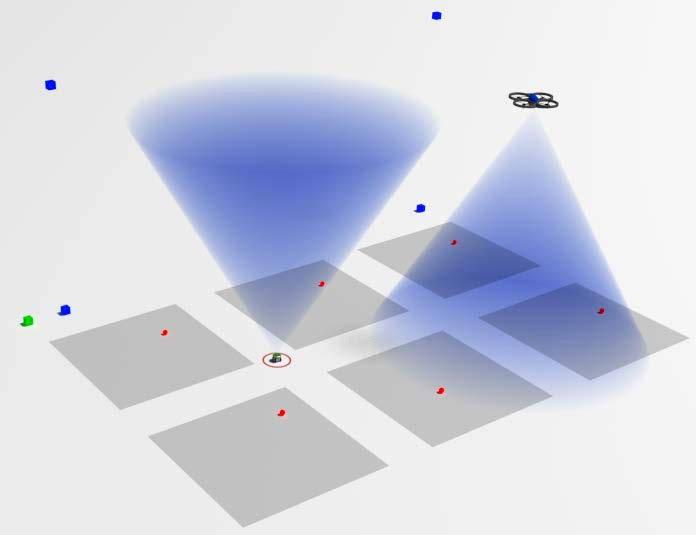
\includegraphics[width=0.8\textwidth]{gomes-fig-1}

\caption{
Figure 1 from \cite{gomes2015cooperative}.
}

\end{figure}

\end{frame}

\begin{frame}{Problem Description}

{\Large
\textbf{minimal prerequisite for meaningful cooperation}
}

\vspace{1ex}

\begin{columns}
\begin{column}{0.02\textwidth}
\end{column}
\begin{column}{0.02\textwidth}
\Huge
\[
\bm{\Bigg\Updownarrow}
\]
\end{column}
\begin{column}{0.96\textwidth}
\begin{itemize}
\item[] \textit{Fix-Tog} --- Fixed altitude, start together
\item[] \textit{Fix-Sep} --- Fixed altitude, start separate
\item[] \textit{Var-Tog} --- Variable altitude, start together
\item[] \textit{Var-Sep} --- Variable altitude, start separate
\end{itemize}
\end{column}
\end{columns}

\vspace{1ex}

{\Large
\textbf{difficult prerequisite for meaningful cooperation}
}

\end{frame}

\begin{frame}{Treatments}

\Large
\begin{itemize}
\item \textit{Base} ---  base CCEA
\item \textit{Inc} --- incremental evolution
\item \textit{NInc} --- non-cooperative incremental evolution
\item \textit{NS} --- novelty-driven coevolution
\end{itemize}
\end{frame}

\begin{frame}{Results}

\begin{figure}
\begin{columns}
\begin{column}{0.5\textwidth}
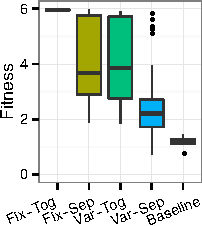
\includegraphics[width=\textwidth]{gomes-fig-2-b}
\end{column}
\begin{column}{0.5\textwidth}
\caption{
Right column of Figure 2 from \cite{gomes2015cooperative}.
}
\end{column}
\end{columns}
\end{figure}

\end{frame}

\begin{frame}{Results}

\begin{figure}

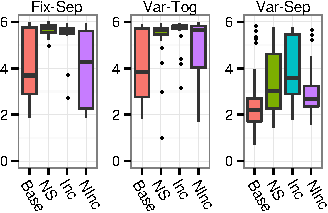
\includegraphics[width=\textwidth]{gomes-fig-3-b}

\caption{
Right column of Figure 3 from \cite{gomes2015cooperative}.
}

\end{figure}

\end{frame}

\begin{frame}{Discussion}

\end{frame}


\section{Genetic team composition and level of selection in the evolution of cooperation \cite{waibel2009genetic}}

\begin{frame}{Problem Description}

\begin{figure}
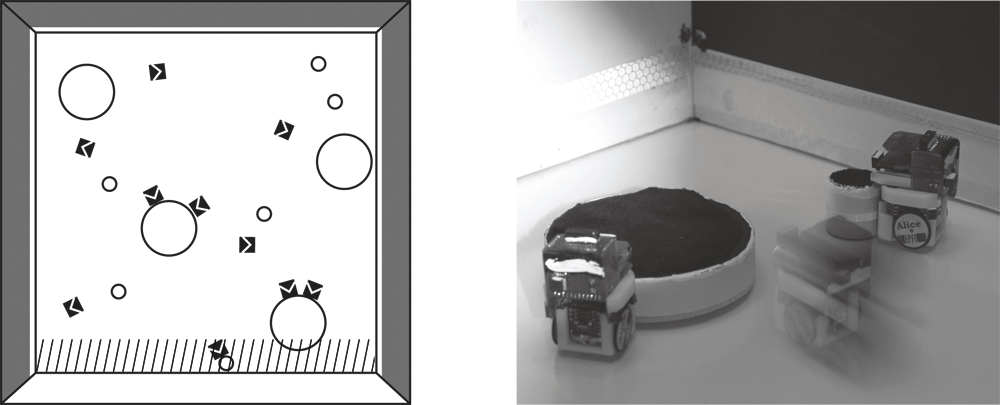
\includegraphics[width=\textwidth]{waibel-fig-3}
\vspace{1ex}
\caption{
Figure 3 from \cite{waibel2009genetic}.
}
\end{figure}

\end{frame}

\begin{frame}{Problem Description}

\textit{Altruistic Cooperative Foraging}
\begin{itemize}
\item six small pucks (1 pt ea to collector)
\item four large pucks (1 pt ea to everybody)
\end{itemize}

\textbf{other tasks:}

\textit{Individual Foraging}
\begin{itemize}
\item six small pucks
\end{itemize}

\textit{Cooperative Foraging}
\begin{itemize}
\item four large pucks
\end{itemize}

\end{frame}


\begin{frame}{Treatments}

\begin{figure}
\begin{columns}
\begin{column}{0.7\textwidth}
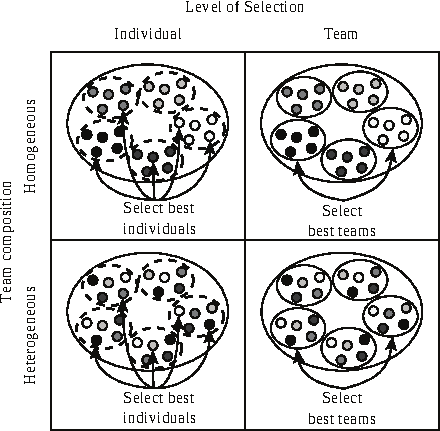
\includegraphics[width=\textwidth]{waibel-fig-2}
\end{column}
\begin{column}{0.3\textwidth}
\caption{
Figure 2 from \cite{waibel2009genetic}.
}
\end{column}
\end{columns}
\end{figure}

\end{frame}

\begin{frame}{Results}

\begin{figure}
\begin{columns}
\begin{column}{0.7\textwidth}
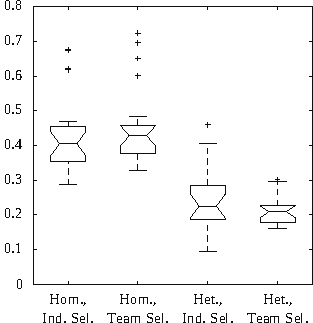
\includegraphics[width=\textwidth]{waibel-fig-9-b}
\end{column}
\begin{column}{0.3\textwidth}
\caption{
Right column of Figure 9 from \cite{waibel2009genetic}.
}
\end{column}
\end{columns}
\end{figure}

\end{frame}

\begin{frame}{Results}


\begin{figure}
\begin{columns}
\begin{column}{0.7\textwidth}
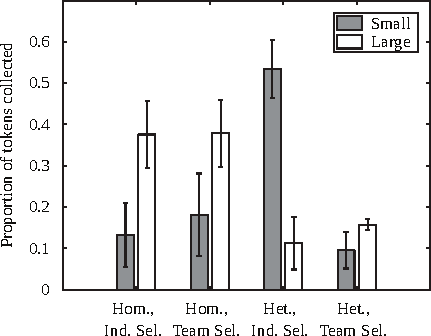
\includegraphics[width=\textwidth]{waibel-fig-10}
\end{column}
\begin{column}{0.3\textwidth}
\caption{
Figure 10 from \cite{waibel2009genetic}.
}
\end{column}
\end{columns}
\end{figure}

\end{frame}

\begin{frame}{Results}

\begin{figure}
\begin{columns}
\begin{column}{0.8\textwidth}
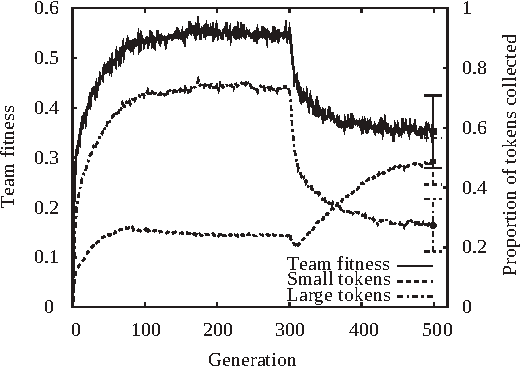
\includegraphics[width=\textwidth]{waibel-fig-12}
\end{column}
\begin{column}{0.2\textwidth}
\caption{
Figure 12 from \cite{waibel2009genetic}.
}
\end{column}
\end{columns}
\end{figure}

\end{frame}

\begin{frame}{Discussion}

directly rewarding large token collection helps address defecting behavior caused by credit-assignment problem under \textit{het., ind. sel}

Figure 12 from \cite{waibel2009genetic} suggests evolutionary contingency not responsible for \textit{het., ind. sel} defecting behavior

weakness: not immediately generalizable to other problem domains
\begin{itemize}
\item e.g., extremely poor performance of local selection treatment in \cite{knudson2010coevolution}
\item requires domain knowledge
\end{itemize}

\end{frame}


\section{Coevolution of heterogeneous multi-robot teams \cite{knudson2010coevolution}}

\begin{frame}{Problem Description}

\begin{figure}

\begin{columns}
\begin{column}{0.7\textwidth}
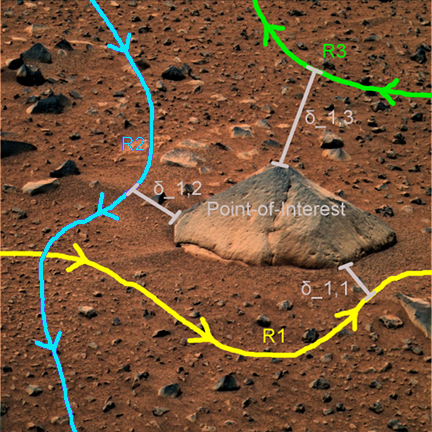
\includegraphics[width=\textwidth]{knudson-fig-2}
\end{column}
\begin{column}{0.3\textwidth}
\caption{
Figure 2 from \cite{knudson2010coevolution}.
}
\end{column}
\end{columns}
\end{figure}

\end{frame}

\begin{frame}{Treatments}
\Large
\begin{itemize}
\item system
\begin{itemize}
\item selection $\sim$ group performance
\end{itemize}
\item local
\begin{itemize}
\item selection $\sim$ \# waypoints an individual visited
\end{itemize}
\item difference
\begin{itemize}
\item selection $\sim$ group performance $-$ group performance w/o individual
\end{itemize}
\item random
\begin{itemize}
\item control treatment
\end{itemize}
\end{itemize}

\end{frame}

\begin{frame}{Results}

\begin{figure}

\begin{columns}
\begin{column}{0.7\textwidth}
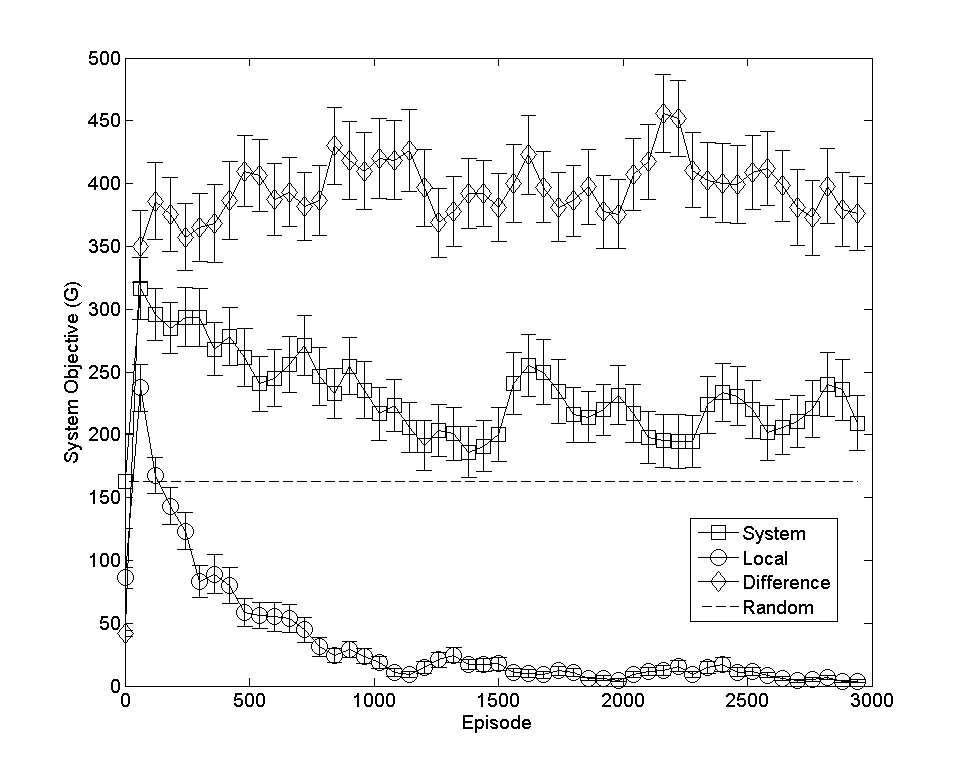
\includegraphics[width=\textwidth]{knudson-fig-7-a}
\end{column}
\begin{column}{0.3\textwidth}
\caption{
Left column of Figure 7 from \cite{knudson2010coevolution}.
}
\end{column}
\end{columns}

\end{figure}

\end{frame}

% \begin{frame}{Results}
%
% \begin{figure}
%
% \begin{columns}
% \begin{column}{0.7\textwidth}
% 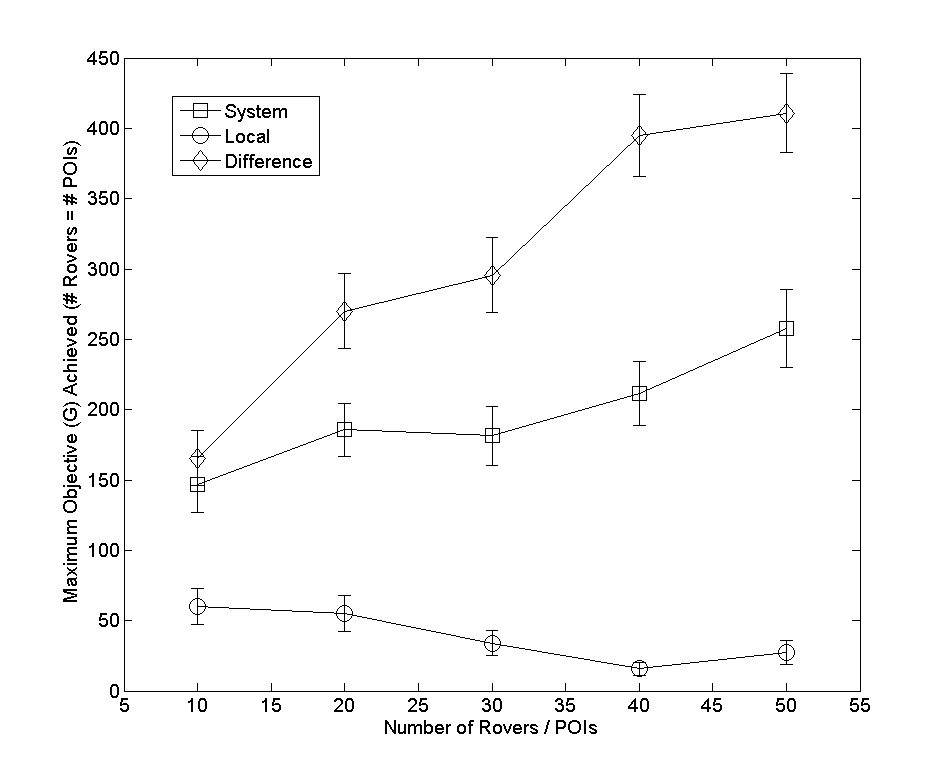
\includegraphics[width=\textwidth]{knudson-fig-7-b}
% \end{column}
% \begin{column}{0.3\textwidth}
% \caption{
% Right column of Figure 7 from \cite{knudson2010coevolution}.
% }
% \end{column}
% \end{columns}
%
% \end{figure}
%
% \end{frame}

\begin{frame}{Discussion}

difference metric is (in principle) generalizable to other problem domains

however, with large groups and without shortcuts it could become computationally prohibitive

assumption for shortcut:
effect of agent on other agents is negligible compared to direct effect of agent on objective

concern:
difference metric might break down in some cases with extreme specialization
\begin{itemize}
\item specifically, when team performance is varyingly sensitive to different team roles
\end{itemize}


\end{frame}

\begin{frame}{Discussion}

How much does team score decrease when removing a sweeper versus removing the thrower?

\begin{figure}
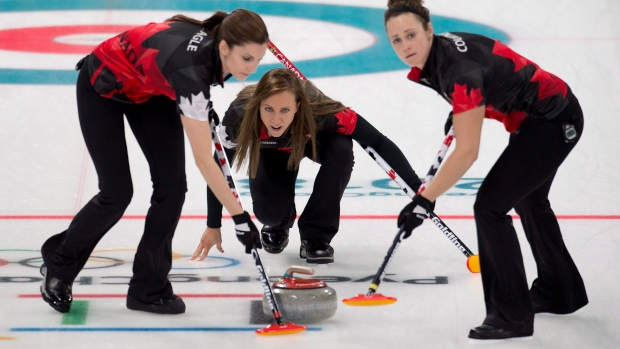
\includegraphics[width=\textwidth]{curling-team}
\caption{A curling team in action.}
\label{fig:curling-team}
\end{figure}

\end{frame}


\section{Synthesis}

\begin{frame}{Aspects of the Credit Assignment Problem}
\begin{itemize}
\item weakening selection \cite{knudson2010coevolution, waibel2009genetic}
\item incentivizing defection \cite{knudson2010coevolution, waibel2009genetic}
\item context dependence \cite{gomes2015cooperative}
\end{itemize}
\end{frame}

\begin{frame}{Problem-specific Knowledge}

difference metric \cite{knudson2010coevolution}
\begin{itemize}
\item employed computational shortcut assumes negligible effects of agent on behavior of other agents
\end{itemize}

reward individual-specific deliverables \cite{waibel2009genetic}
\begin{itemize}
\item depends on rewarded individual-specific deliverables aligning with group performance
\end{itemize}

cooperative co-evolution \cite{gomes2015cooperative}
\begin{itemize}
\item need to define expected cooperating roles \textit{a priori}
\end{itemize}

\end{frame}

\begin{frame}{Team Genome}
idea: bypass credit-assignment problem altogether by evolving teams as a unit

\begin{itemize}
\item completely clonal group
\begin{itemize}
\item lose out on configuration specialization
\end{itemize}
\item completely non-clonal group
\begin{itemize}
\item too many parameters
\end{itemize}
\item partially clonal group \cite{bongard2000legion}
\begin{itemize}
\item analogy: indirect encoding that exploits symmetries to simplify the genetic search space \cite{bongard2000legion}
\end{itemize}
\item need domain knowledge about team size?
\begin{itemize}
\item try evolving team size \cite{bongard2000legion}
\end{itemize}

\end{itemize}

\end{frame}

\begin{frame}{Inspiration from Nature}

\begin{columns}
\begin{column}{0.5\textwidth}
hypothesized mechanisms that stabilize cooperation between genetically-dissimilar individuals \cite{vostinar2017suicide, andre2016evolutionary}:
\begin{itemize}
\item transitions of individuality
\item vertical transmission
\item partner selection
\item reciprocity
\end{itemize}
\end{column}
\begin{column}{0.5\textwidth}
\begin{figure}
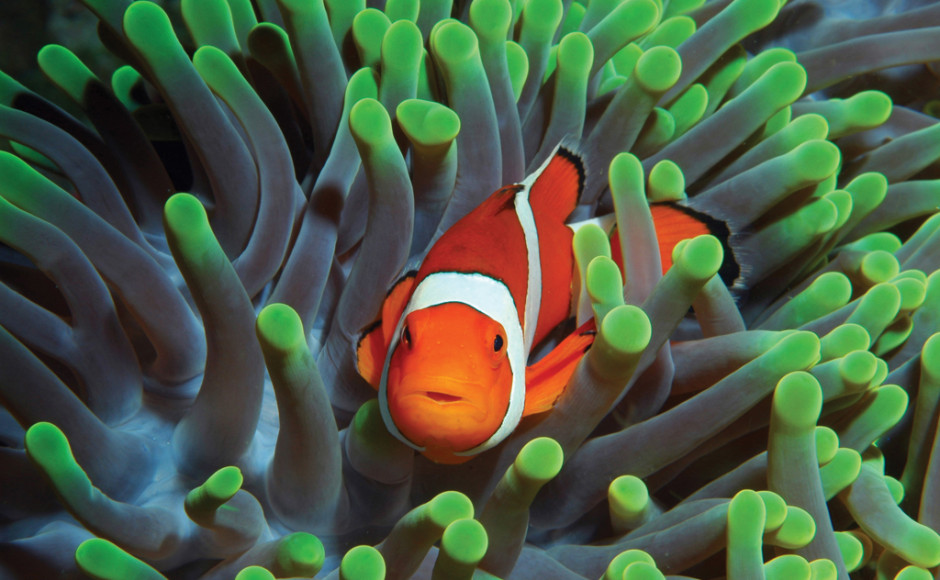
\includegraphics[width=\textwidth]{clownfish}
\caption{
Clownfish and sea anenomones have a symbiotic relationship \cite{dunn1981clownfish}.
}
\label{fig:clownfish}
\end{figure}
\end{column}
\end{columns}
\end{frame}


\appendix

\begin{frame}{Acknowledgements}
\begin{itemize}
\item Charles Ofria (advisor)
\item Wolfgang Banzhaf (committee member)
\item Anil Jain (committee member)
\item Kevin Liu (committee member)
\item Eric Torng (exam coordinator)
\end{itemize}
\vspace{-1ex}

\newcommand{\innerspacer}{0.1\textwidth}
\newcommand{\content}{0.3\textwidth}
\newcommand{\outerspacer}{0.15\textwidth}


\begin{center}
 \begin{columns}
	\begin{column}{\outerspacer}~\end{column}
	 \begin{column}{\content}
		\includegraphics[width=\textwidth]{BEACON-logo}
 	\end{column}
  \begin{column}{\innerspacer}~\end{column}
 	\begin{column}{\content}
   \includegraphics[width=\textwidth]{MSU-helmet}
 	\end{column}
 	\begin{column}{\outerspacer}~\end{column}
 \end{columns}
\end{center}

\end{frame}

\begin{frame}[allowframebreaks]{Image Sources}

\footnotesize

Figure
\ref{fig:professional-hockey}:
\url{
https://www.sportsnet.ca/olympics/hockey-canada-announces-2018-olympic-womens-hockey-team/
}

Figure
\ref{fig:amateur-hockey}:
\url{
https://discoverhometown.com/washington-county-youth-hockey-team-wins-state-title
}

Figure
\ref{fig:crowded-rink}:
\url{
http://www.healthclubmanagement.co.uk/health-club-management-news/Floating-ice-rink-brings-Raiders-back-to-Romford-at-new-%C2%A328m-leisure-centre/336337
}

Figure
\ref{fig:slap-shot}:
\url{
https://thehockey411.com/2017/02/09/on-the-wrong-end-of-a-slap-shot/
}

Figure
\ref{fig:royal-road-pass}:
\url{
https://www.msgnetworks.com/2015/03/06/the-royal-road-to-the-future-of-goaltender-analytics/
}

\end{frame}

\begin{frame}[standout]
  Questions?
\end{frame}

\begin{frame}[allowframebreaks]{References}

  \bibliography{bibl}
  \setbeamertemplate{bibliography item}{\insertbiblabel}
  %\nocite{*} % Insert publications even if they are not cited in the poster
  \bibliographystyle{apalike}
\end{frame}


% \input{tex/backup.tex}

\end{document}
